% Page 031 — page imprimée 27
% Contenu seul : le préambule et la pagination sont gérés par meyrueis.tex

Au carrefour de nos vallées étroites toute cette vie se mêle et se confond, ces deux génies de
la montagne, l’un de granit, l’autre de calcaire, nous observent, nous inquiètent et nous
protègent.

Ils détiennent le pouvoir de l’eau ; haut placés, ils captent les nuages et chacun d’entre nous
les renvoie à sa façon : le Causse boit l’eau goulûment et la rejette au bas de la falaise, tandis
que l’Aigoual la laisse couler à l’air libre sur des kilomètres, tout le long des vallées.

Ici, l’eau joue un grand rôle : avalée par les avens, calcifiée dans les grottes, creusant des
gorges célèbres. Pour nous, cela est naturel, nous l’avons toujours vu.

Paradoxalement, nos émotions les plus fortes nous les avons ressenties avec les sources, ces
jaillissements spontanés, imprévus, connus des seuls initiés.

Des sources il y en a partout dans les vallées : celle du Pied Pointu qui sort à deux pas du ciel,
est directement branchée sur les nuages ; les bergers ont mis quatre pierres pour la retenir un
peu. Seuls quelques myosotis et une végétation insolite la trahissent ; elle est là, silencieuse,
moqueuse, elle passe directement du ciel au ventre de la terre.

Il y a la « gourguette » qui jaillit au bord de la route pour le passant, « la fontaine de
Paul » qui sort presque dans la rivière, celle du « serre » bien placée pour les moissonneurs et
le troupeau et que l’on surveille de près de peur de la perdre...

Et puis un jour, nous avons remonté la vallée de schiste bleu jusqu’à l’horizon ouvert, jusqu’à
la source de la rivière. Toute une journée nous avons arpenté forêts et pâturages.

Et, là-haut, nous avons connu le granit, ces grosses boules belles comme des bijoux,
imbriquées en jeu de construction monumentaux, piédestal des rapaces.

Nous avons rencontré le troupeau transhumant. Il enroulait et déroulait son chemin de laine et
le mouton disparaissait dans le troupeau vivant.

Le soir nous avons couché au sommet pour assister au lever du soleil car ici, l’arrivée du jour
est un moment rare, mais le soleil, dans les brumes, n’est apparu qu’à dix heures, frileux et
moqueur....

Ce jour-là, nous avions déchiré un petit bout du mystère de l’Aigoual.

\begin{flushright}
Janine BRAGER
\end{flushright}

\begin{flushright}
Extraits de « Cévennes et Grands Causses »\\
d’Alain Gas Presses du Languedoc p.13-14
\end{flushright}

\vspace{0.6em}

\begin{center}
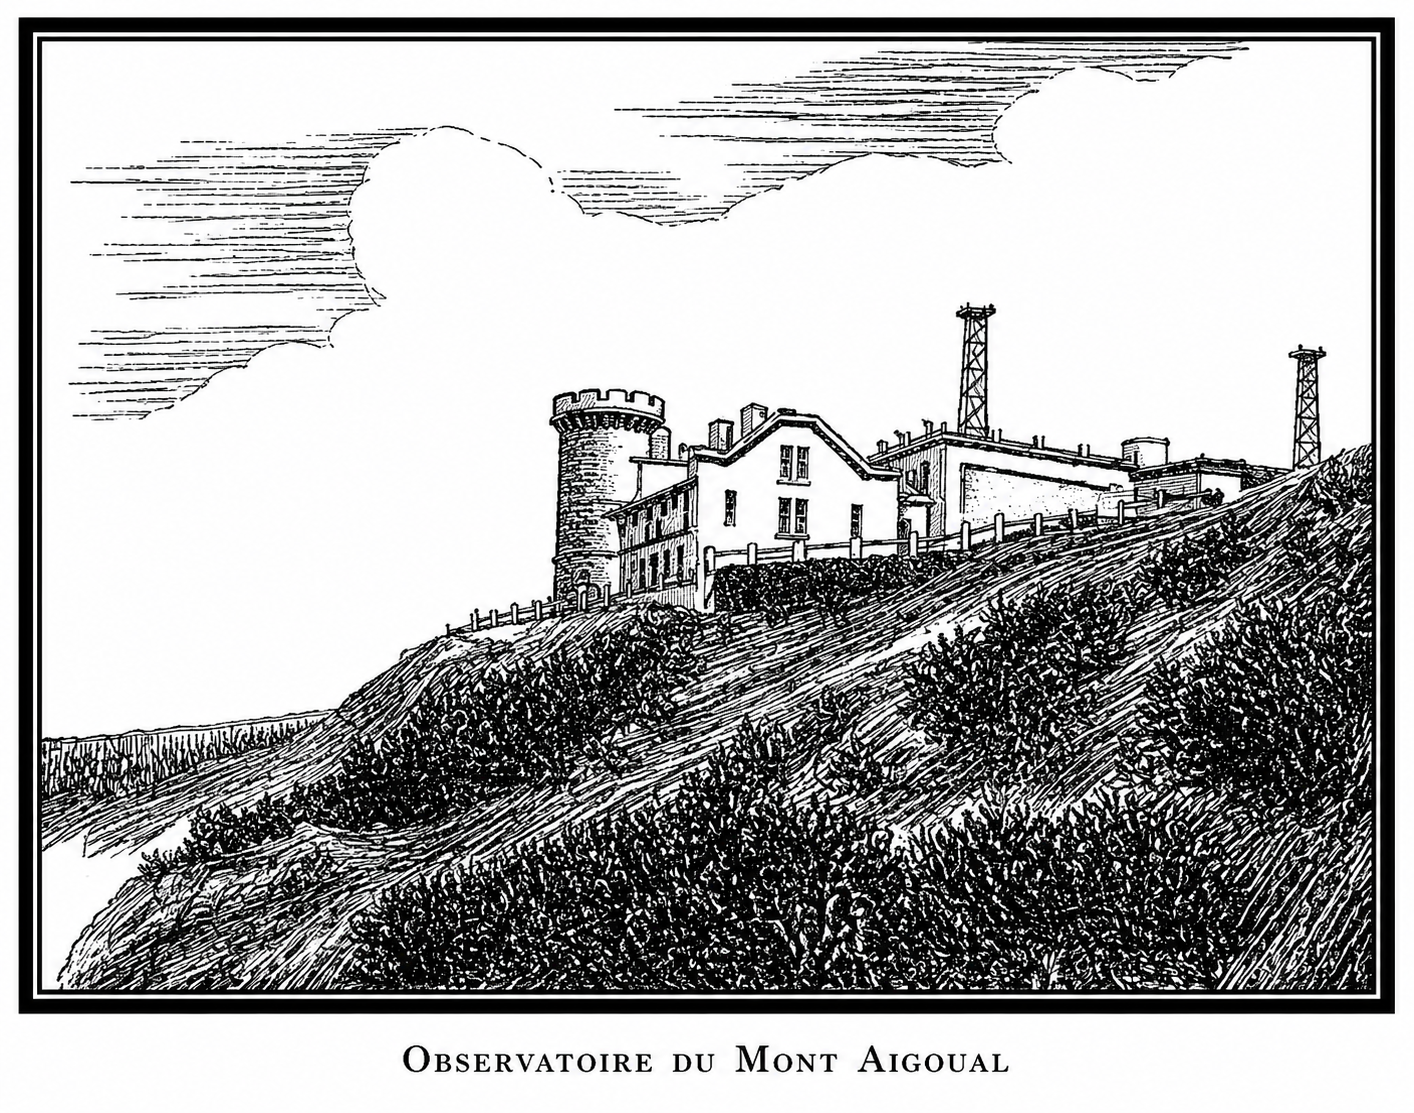
\includegraphics[width=0.63\textwidth]{imgs/031.png}
\end{center}
